\documentclass{article}
\usepackage[utf8]{inputenc}

\title{Project 3}
\author{Ryan Wood\\
rwood@college.harvard.edu}
\date{May 2018}

\usepackage{tikz}
\usepackage{amsmath}
\usetikzlibrary{arrows}
\usepackage{natbib}
\usepackage{graphicx}
\usepackage{amsmath}
\usepackage{enumerate}
\usepackage[margin=1.4in]{geometry}
\usepackage{fancyhdr}
\usepackage{pgfplots}
\pagestyle{fancy}
\lhead{Dr. Chen}
\chead{Project 3}
\rhead{Ryan Wood}

\begin{document}
\maketitle

\section{Regression: Predicting Age from Small Subset of BIFs}
\begin{enumerate}[a)]
\item \textbf{Linear Regression of Age from One BIF Predictor}

After importing ID and minimum age data, we can use R's `linear models' function to fit the first BIF and the corresponding minimum age:\\
\begin{verbatim}
# import ID vector and min age vector
IDs = read.csv('/Users/ryanwood/Documents/Summer 2018 - UNCW /Project 2-May 23, 2018/IDs.csv')
IDs = unlist(IDs$x)
minAges = read.csv('/Users/ryanwood/Documents/Summer 2018 - UNCW /Project 2-May 23, 2018/minAges.csv')
minAges = unlist(minAges$x)

# take only first 20 BIFs
BIFData1 = BIFData[,1:21]
# extract the IDs
BIFData1$V1 = as.character(BIFData1$V1)
for (ii in 1:length(BIFData[,1])) {
  BIFData1$V1[ii] = substr(as.character(BIFData1[ii,1]),1,6)
}
# make vector with min ages corresponding to BIF data
BIFages = unlist(as.numeric(BIFData1$V1))
for (ii in 1:length(BIFages)) {
  tmpIndex = match(BIFages[ii],IDs)
  BIFages[ii] = minAges[tmpIndex]
}

### linear regression
attach(BIFData1[,2:length(BIFData1[1,])])
lm.fit = lm(BIFages~V2)
summary(lm.fit)
coef(lm.fit)
plot(V2,BIFages,main='Linear Regression of First 20 BIFs')
abline(lm.fit$coefficients[1],lm.fit$coefficients[2])
\end{verbatim}

The resulting regression has the following properties:\\
\begin{verbatim}
Residuals:
    Min      1Q  Median      3Q     Max 
-20.072  -8.942  -1.139   7.943  33.988 

Coefficients:
             Estimate Std. Error t value Pr(>|t|)    
(Intercept) 22.461869   1.347631  16.668  < 2e-16 ***
V2           0.055778   0.007958   7.009 4.41e-12 ***
---
Signif. codes:  0 ?***? 0.001 ?**? 0.01 ?*? 0.05 ?.? 0.1 ? ? 1

Residual standard error: 10.85 on 998 degrees of freedom
Multiple R-squared:  0.04692,	Adjusted R-squared:  0.04596 
F-statistic: 49.13 on 1 and 998 DF,  p-value: 4.412e-12
\end{verbatim}
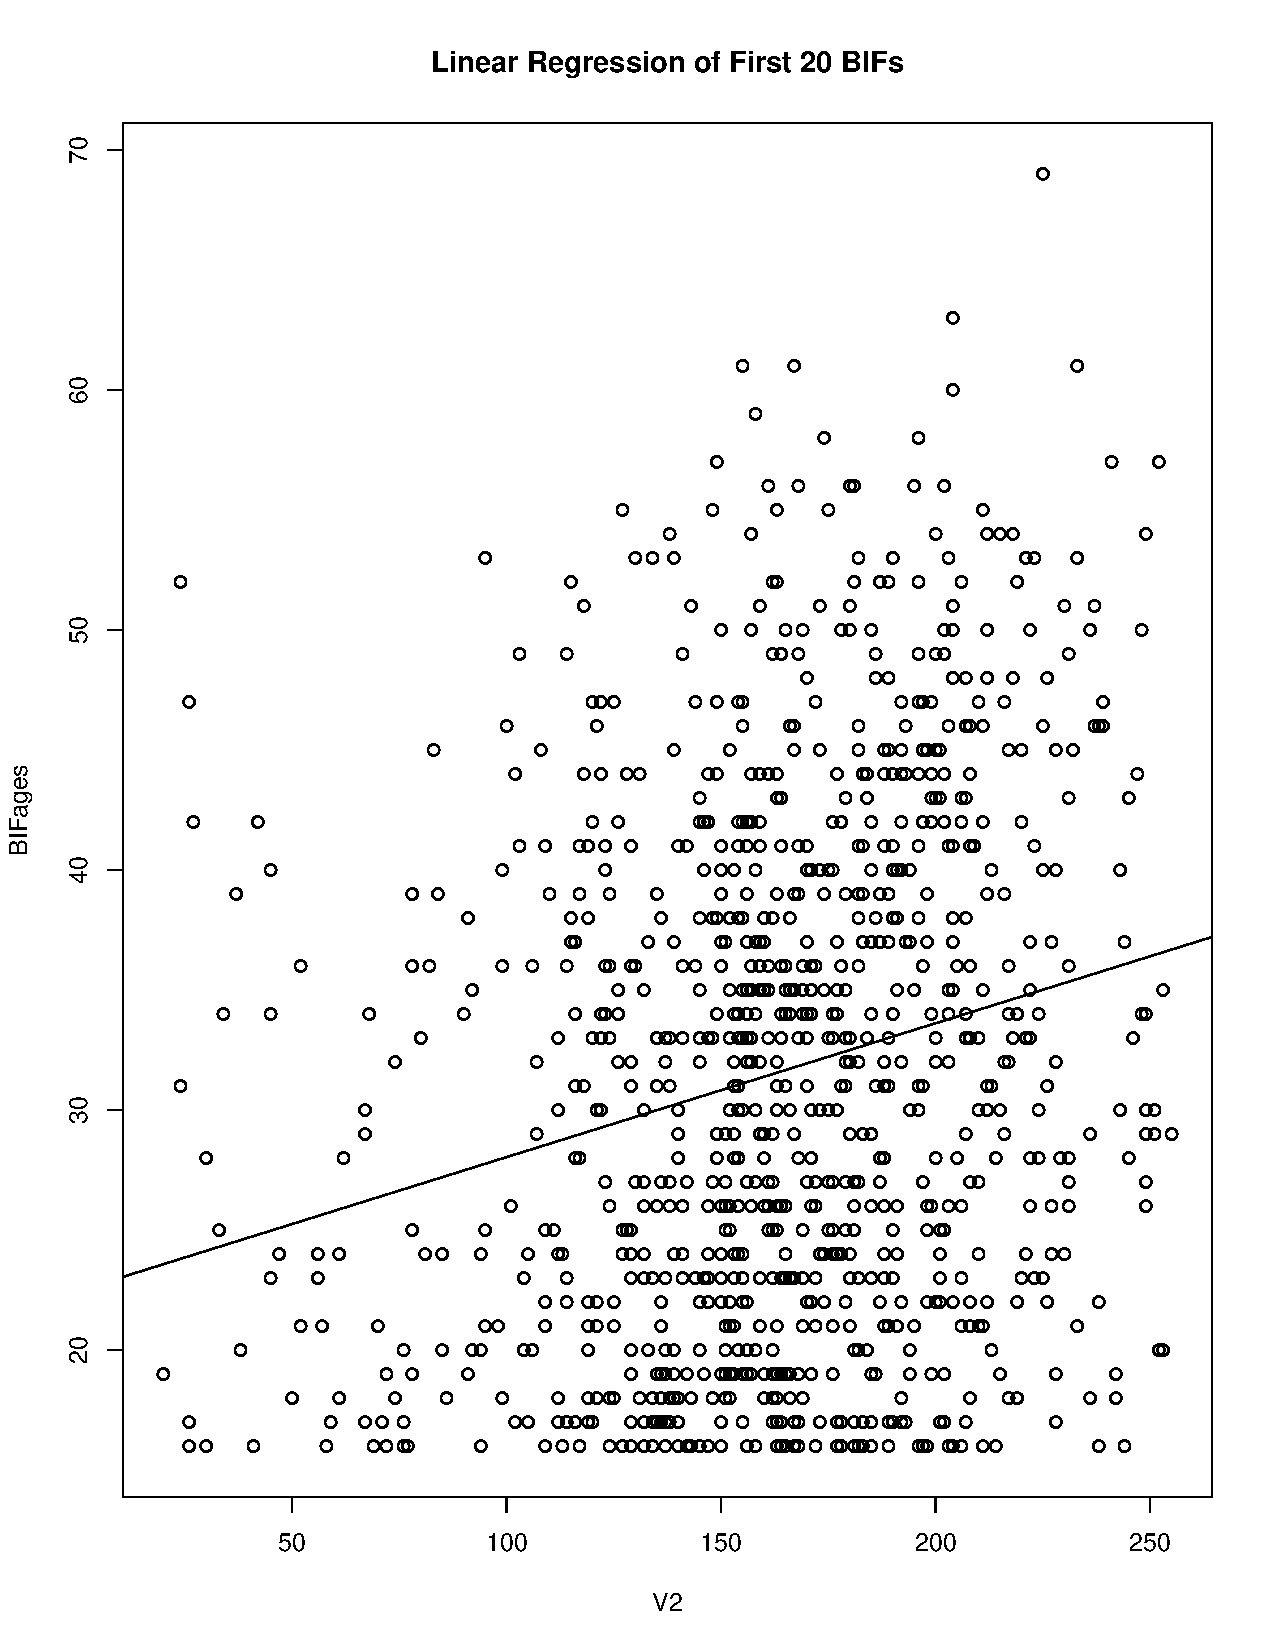
\includegraphics[width=0.4\textwidth]{E1a.pdf}\\

\item \textbf{Quadratic Regression of Age from One BIF Predictor}
\begin{verbatim}
### quadratic regression
lm.fit2 = lm(BIFages~poly(V3,2))
summary(lm.fit2)
plot(V3,BIFages,main='Quadratic Regression of First 20 BIFs')
x = seq(0,255,length=100)
lines(x,predict(lm.fit2,data.frame(V3=x)),col="blue")
\end{verbatim}
The results are as follows:\\
\begin{verbatim}
Residuals:
    Min      1Q  Median      3Q     Max 
-19.383  -9.386  -0.894   8.044  34.365 

Coefficients:
             Estimate Std. Error t value Pr(>|t|)    
(Intercept)   31.5960     0.3465  91.177  < 2e-16 ***
poly(V3, 2)1  58.5747    10.9583   5.345 1.12e-07 ***
poly(V3, 2)2  14.2353    10.9583   1.299    0.194    
---
Signif. codes:  0 ?***? 0.001 ?**? 0.01 ?*? 0.05 ?.? 0.1 ? ? 1

Residual standard error: 10.96 on 997 degrees of freedom
Multiple R-squared:  0.02946,	Adjusted R-squared:  0.02751 
F-statistic: 15.13 on 2 and 997 DF,  p-value: 3.366e-07
\end{verbatim}
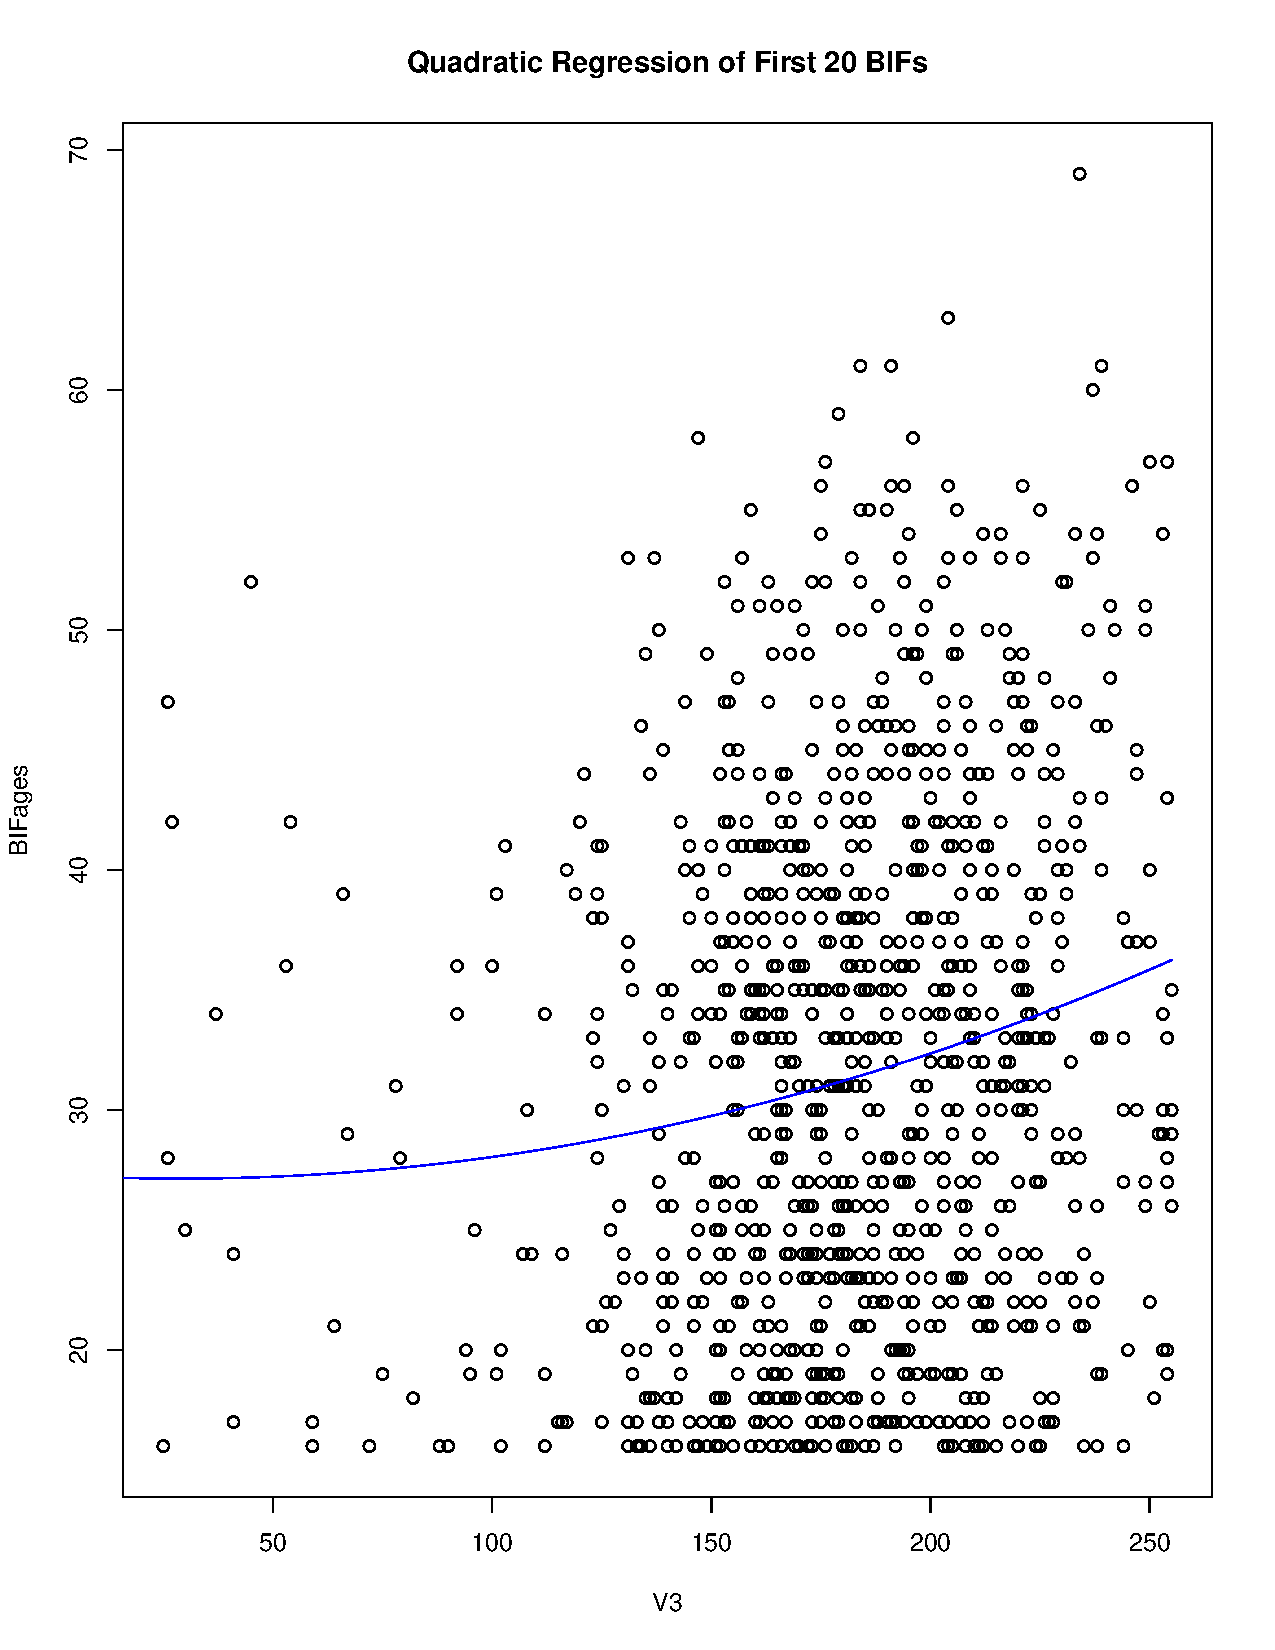
\includegraphics[width=0.4\textwidth]{E1b.pdf}\\

\item \textbf{Polynomial Regression of Age from One BIF Predictor}
\begin{verbatim}
## cubic regression
lm.fit3 = lm(BIFages~poly(V3,3))
summary(lm.fit3)
plot(V3,BIFages,main='Cubic Regression of First 20 BIFs')
x = seq(0,255,length=100)
lines(x,predict(lm.fit3,data.frame(V3=x)),col="red")
\end{verbatim}
The results are as follows:\\
\begin{verbatim}
Residuals:
    Min      1Q  Median      3Q     Max 
-18.342  -9.264  -1.019   7.976  34.735 

Coefficients:
             Estimate Std. Error t value Pr(>|t|)    
(Intercept)   31.5960     0.3461  91.297  < 2e-16 ***
poly(V3, 3)1  58.5747    10.9440   5.352 1.08e-07 ***
poly(V3, 3)2  14.2353    10.9440   1.301   0.1936    
poly(V3, 3)3 -20.8267    10.9440  -1.903   0.0573 .  
---
Signif. codes:  0 ?***? 0.001 ?**? 0.01 ?*? 0.05 ?.? 0.1 ? ? 1

Residual standard error: 10.94 on 996 degrees of freedom
Multiple R-squared:  0.03297,	Adjusted R-squared:  0.03006 
F-statistic: 11.32 on 3 and 996 DF,  p-value: 2.638e-07
\end{verbatim}
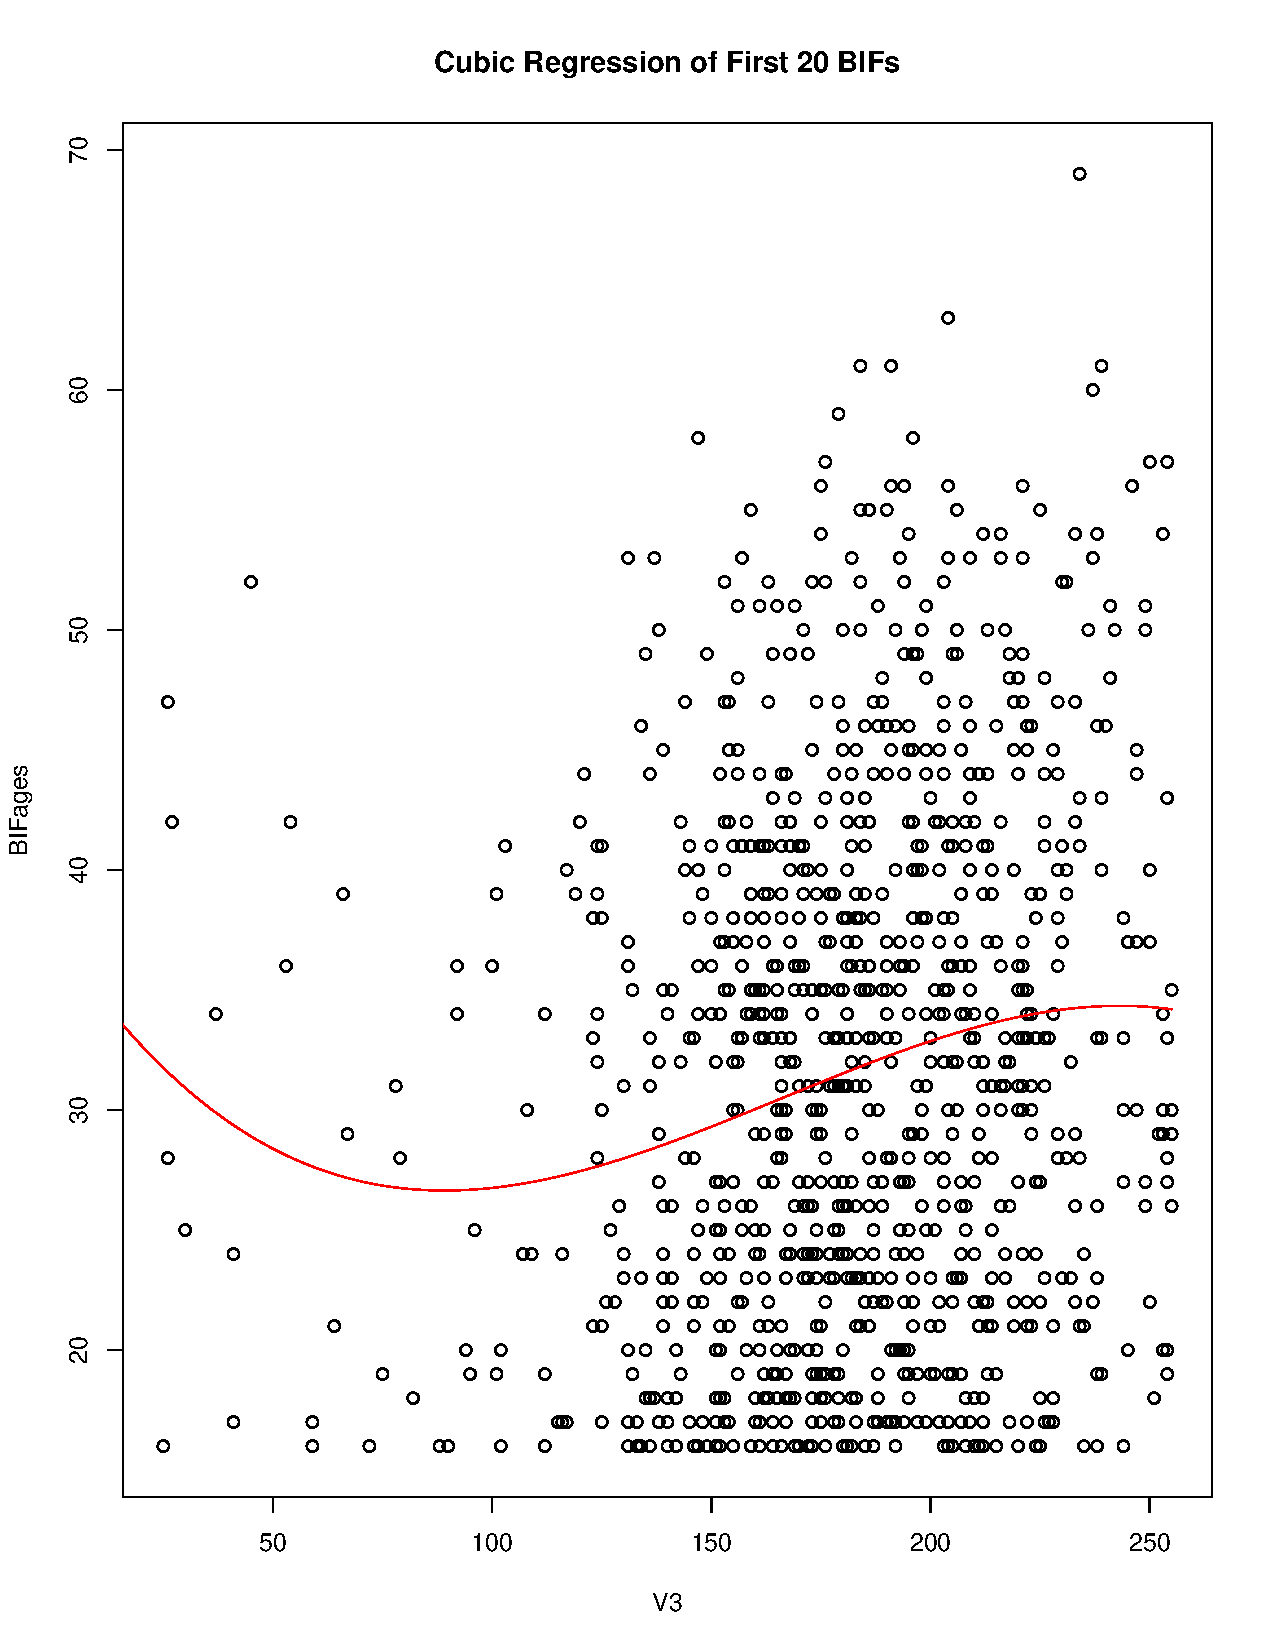
\includegraphics[width=0.4\textwidth]{E1c.pdf}\\

\end{enumerate}

\section{Classification: Predicting Gender and Race from Full BIF Dataset}
The first thing we need to do is import the BIF data and gender data.\\
\begin{verbatim}
rm(list=ls())
dev.off()
BIFData = read.csv("/Users/ryanwood/Documents/Summer 2018 - UNCW /Project 1-May 22, 2018/MorphII_BIF_s7-37_g0.1_max_partial.csv",header = F);
# make labels vector for gender, 1 for female and 0 for male
genderLabels = rep(0,length(BIFgenders))
for (ii in 1:length(genderLabels)) {
  if (BIFgenders[ii] == "F") {
    genderLabels[ii] = 1
  }
}
\end{verbatim}
\begin{enumerate}[a)]
\item \textbf{Logistic Regression}
\begin{verbatim}
# train the model
glm.fit=glm(genderLabels~.-V1,data=BIFData[,1:150],family=binomial)

# predict using training data
glm.predictions = predict(glm.fit,type="response")
glm.predictions[glm.predictions<0.5] = 0
glm.predictions[glm.predictions>=0.5] = 1

# confusion table
confusionTable = table(glm.predictions,genderLabels)
confusionTable

# overall accuracy
accuracy=mean(genderLabels==glm.predictions)

# sensitivity (portion of 1's correctly predicted)
sensitivity=confusionTable[4]/(confusionTable[4]+confusionTable[3])

# specificity (portion of 0's correctly predicted)
specificity=confusionTable[1]/(confusionTable[1]+confusionTable[2])
\end{verbatim}

The confusion table for logistic regression is as follows:\\
\begin{tabular}{l c r}
  & 0 & 1 \\
0 & 825 & 41 \\
1 & 18 & 116 \\
\end{tabular}\\
The overall accuracy was 0.941. The sensitivity was 0.739. The specificity was 0.979.\\


\item \textbf{Linear Discriminant Analysis}
\begin{verbatim}
# train model
lda.fit=lda(genderLabels~.-V2,data=BIFData[,2:150])

# plot the model
plot(lda.fit)

# predict using training data
lda.predictions = predict(lda.fit,BIFData[,2:150],type="response")
lda.predictions = lda.predictions$class

# confusion table
confusionTable = table(lda.predictions,genderLabels)
confusionTable

# overall accuracy
accuracy=mean(genderLabels==lda.predictions)

# sensitivity (portion of 1's correctly predicted)
sensitivity=confusionTable[4]/(confusionTable[4]+confusionTable[3])

# specificity (portion of 0's correctly predicted)
specificity=confusionTable[1]/(confusionTable[1]+confusionTable[2])
\end{verbatim}

The confusion table for LDA is as follows:\\
\begin{tabular}{l c r}
  & 0 & 1 \\
0 & 825 & 53 \\
1 & 28 & 104 \\
\end{tabular}\\
The overall accuracy was 0.919. The sensitivity was 0.662. The specificity was 0.967.\\

\item \textbf{Quadratic Discriminant Analysis}
\begin{verbatim}
# train model
qda.fit=qda(genderLabels~.-V2,data=BIFData[,2:50])

# plot the model
plot(qda.fit)

# predict using training data
qda.predictions = predict(qda.fit,BIFData[,2:50],type="response")
qda.predictions = qda.predictions$class

# confusion table
confusionTable = table(qda.predictions,genderLabels)
confusionTable

# overall accuracy
accuracy=mean(genderLabels==qda.predictions)

# sensitivity (portion of 1's correctly predicted)
sensitivity=confusionTable[4]/(confusionTable[4]+confusionTable[3])

# specificity (portion of 0's correctly predicted)
specificity=confusionTable[1]/(confusionTable[1]+confusionTable[2])
\end{verbatim}
The confusion table for QDA is as follows:\\
\begin{tabular}{l c r}
  & 0 & 1 \\
0 & 814 & 70 \\
1 & 29 & 67 \\
\end{tabular}\\
The overall accuracy was 0.901. The sensitivity was 0.554. The specificity was 0.966.\\


\item \textbf{K Nearest Neighbors}
\begin{verbatim}
# train/predict model
knn.predictions = knn(BIFData[,2:150],BIFData[,2:150],genderLabels,k=3)

# confusion table
confusionTable = table(knn.predictions,genderLabels)
confusionTable

# overall accuracy
accuracy=mean(genderLabels==knn.predictions)

# sensitivity (portion of 1's correctly predicted)
sensitivity=confusionTable[4]/(confusionTable[4]+confusionTable[3])

# specificity (portion of 0's correctly predicted)
specificity=confusionTable[1]/(confusionTable[1]+confusionTable[2])
\end{verbatim}
The confusion table for QDA is as follows:\\
\begin{tabular}{l c r}
  & 0 & 1 \\
0 & 829 & 77 \\
1 & 14 & 80 \\
\end{tabular}\\
The overall accuracy was 0.909. The sensitivity was 0.510. The specificity was 0.983.\\



\end{enumerate}
\end{document}
